\documentclass[smallheadings,12pt]{scrartcl}
%\usepackage{marvosym}
\usepackage{color}
\usepackage{float}
\usepackage{geometry}
\usepackage{graphicx}
\usepackage{soul} % underlining text
\geometry{verbose,letterpaper,tmargin=2cm,bmargin=3cm,lmargin=2.5cm,rmargin=3.5cm}
\usepackage[utf8]{inputenc}
\usepackage[dvips,bookmarks,colorlinks=true]{hyperref}
%\usepackage[bookmarks,colorlinks=true]{hyperref}
\usepackage{listings}

\usepackage[english]{babel}
%\documentclass[normalheadings,twocolumn,12pt]{scrartcl}
%\usepackage{mysty}
\usepackage{amsmath}
\usepackage{amsfonts}
\usepackage{amssymb}
\newcommand{\skills}[1]{\rule{1cm}{0pt}{\begin{minipage}{.8\textwidth}\small\em
      Learned Skills:  #1\end{minipage}}}

	  
\newenvironment{packed_item}{
\begin{itemize}
  \setlength{\itemsep}{1pt}
  \setlength{\parskip}{0pt}
  \setlength{\parsep}{0pt}
}{\end{itemize}}	  
	  
%----------------------------------------
\newcommand{\pd}[2]{\frac{\partial #1}{\partial #2}}
\DeclareMathOperator*{\sgn}{sgn}
\DeclareMathOperator*{\sig}{sig}
\DeclareMathOperator*{\argmin}{arg\,min}
\DeclareMathOperator*{\argmax}{arg\,max}
%--------------------------------------


\begin{document}
\parindent0cm
%\pagestyle{myheadings}
\title{Python Exercises\\ Introduction - Advanced}
\lstset{language=Python,numbers=left,frame=shadowbox}
\date{}
\maketitle

\section{Find Errors}
\skills{basic python skills}

Find four programming errors in the below example (if you find five,
win a candy).
\begin{lstlisting}
#!/usr/bin/ env python

import sys, random
def compute(n):
   i = 0; s = 0
   while i <= n:
      s += random.random()
       i += 1
   return s/n

n = sys.argv[1]
print 'the average of %d random numbers is %g' % (n, compute(n))
\end{lstlisting}


\section{Cartesian/Polar Coordinates}
\skills{Writing functions}

Points may be given in polar $(r,\theta)$ or cartesian coordinates
$(x,y)$, see Figure~\ref{fig:pol2cart}.
\begin{figure}[H]
  \centering
  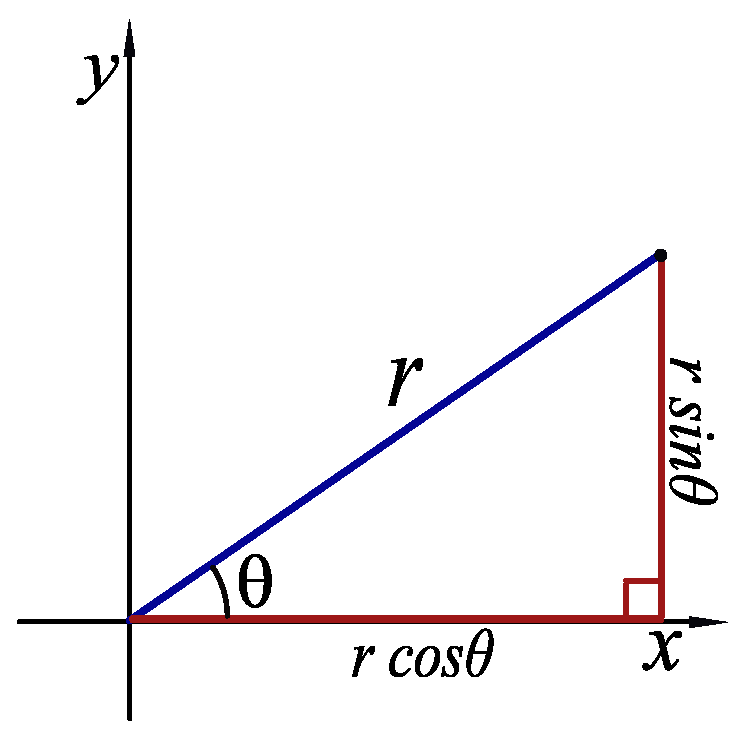
\includegraphics[width=0.25\textwidth]{pics/pol2cart.eps}
  \caption{Relationship between polar and cartesian coordinates.\label{fig:pol2cart}}
\end{figure}

\begin{enumerate}
\item Write a function \texttt{pol2cart}, that takes a tuple $(r,\theta)$ in polar
  coordinates and returns a tuple in cartesian coordinates. 
\item Write the inverse function \texttt{cart2pol}, such that {\tt
  pol2cart(~cart2pol(~(x,y)~)~)} is $(x,y)$ for any input $(x,y)$.
\item Extend the two functions, such that they can in addition handle
  lists of tuples.
\end{enumerate}

\section{Word counting}
\skills{File input/output}
\begin{enumerate}
\item Create a script that opens a text file for reading and report the number of lines,
 words and characters. Assume that words are separated by whitespace (forget hifens!).
\item Open a text file for writing and save the count in it.
\item Extra: Choose a book from The Project Gutenberg
 (\url{www.gutenberg.org}, e.g., \href{http://www.gutenberg.org/cache/epub/964/pg964.txt}{``The Merry Adventures of Robin Hood, by Howard Pyle''}) in
 text format and list the ten most frequently used words. You can use a Dictionary for counting.
\end{enumerate}
\textbf{Useful:} {\tt string.split(), open(), file.read()} and {\tt file.write()}.

\section{Party game}
\skills{Random numbers; Loops}

One guessing game, called ``squeezed'', is very common in
parties. It consists of a player, the chooser,
who writes down a number between 00--99. The other players then take
turns guessing numbers, with a catch: if one says the chosen number,
he loses and has to do something daft. If the guessed number is not the chosen
one, it splits the range. The chooser then states the part which contains
the chosen number. If the new region only has one number, the
chooser is said to be ``squeezed'' and is punished. An example of gameplay would be:
\begin{packed_item}
	\item Chooser writes down (secretly) his number (let's say, 30).
	\item[---] Chooser: ``State a number between 00 and 99.'' 
	\item[---] Player: ``42''.
	\item[---] Chooser: ``State a number between 00 and 42.''
	\item[---] Player: ``26''.
	\item[---] Chooser: ``State a number between 26 and 42.''
	\item[] \hspace{3cm} $\vdots$
	\item[---] Chooser: ``State a number between 29 and 32.''	
	\item[---] Player: ``31''.
	\item Chooser dances some very silly children song.
\end{packed_item}
Implement this game in Python, where the computer is the chooser.\\[2pt]
\textbf{Useful:} {\tt random.randint()} and {\tt raw\_input()}.


\section{Rock-paper-scissors}
\skills{Random choices}

Implement the game of rock-paper-scissors.
Extra: make it {rock-paper-scissors-lizard-spock} (if you do not know it, Wikipedia should help).\\[2pt]
\textbf{Useful:} {\tt random.choice()}.

\section{Dice Simulation}
\skills{Random numbers; Monte-Carlo Simulation}

Estimate the chance of an event in a dice game.  What is the
probability of getting at least one 6 when throwing two dice?  This
question can be analyzed theoretically by methods from probability
theory. However, a more general alternative is to let a computer
program throw two dice a large number of times and count how many
times a 6 shows up. Such type of computer experiments, involving
uncertain events, is often called Monte Carlo simulation. 

\begin{enumerate}
\item Create a script that in a loop from 1 to $n$ draws two uniform
  random integers between 1 and 6 and counts how many times $p$ a 6
  shows up. Write out the estimated probability $p/n$ together with
  the exact result $11/36$.  Run the script a few times with different
  $n$ values and determine from the experiments how large n must be to
  get at least three decimals $(0.306)$ of the probability
  correct.  Use the random module to draw random uniformly distributed
  integers in a specified interval.
\item Generalize the script to an arbitrary number of dices, $N$.
\item Determine if you win or lose a hazard game.  Somebody suggests
  the following game. You pay 1 unit of money and are allowed to throw
  four dice. If the sum of the eyes on the dice is less than 9, you
  win 10 units of money, otherwise you lose your investment. Should
  you play this game?
\end{enumerate}


\section{Run an external script}
\skills{Calling external applications; List handling}

\begin{enumerate}
\item Write a script \texttt{runexternal.py} that runs the
  dice-simulation developed in the last exercise as an external
  program for a range of parameters ($n$ and $N$). The parameters
  should be passed to the script as command-line parameters. Collect
  the result in a list that as each element contains a four-tuple
  ($N$, $n$, result, analytical result).

  Note: You could of course just put a loop into the monte-carlo
  script. However, calling it as an external application gives you the
  opportunity to put any program instead of the Monte-Carlo script
  (say a compiled simulation program you got from a collegue).
  
  Use subprocess.call() for calling the script. Note that the subprocess module is most appropriate to learn because this module intends to replace several other, older modules and functions, such as: "os.system","os.spawn*","os.popen*","popen2.*" and "commands.*".

\item Output the result in a comma-separated (.csv) file.
\item Let {\tt runexternal.py} take command line arguments that allow
  the user to specify ranges in MATLAB-style for which the external
  script should be called.

  E.g. 
\begin{verbatim}
$ python runexternal.py N=1:5 n=100:1000:10000 
\end{verbatim}
should run the script with any combination of $N=1,2,3,4,5$ and
$n=100,1100,2100,\ldots$. 
 
\end{enumerate}


\section{Calculating a Histogram}
\skills{Creating a function; List handling; Random numbers}

\begin{enumerate}
\item Write a function {\tt histgram(data, numbins)} which calculates the
  histogram of a given data set, where {\tt numbins} gives the number of intervals in which the data range is divided.\\
  The function should return a tuple of two lists of equal lengths. The first list contains the midpoints of
  the intervals and the second list contains the
  counts of data points in the interval. 
\item Give a pseudo-graphical representation of the distribution, by
  drawing a number of stars corresponding to the number of
  data elements in a given interval. Example:
\begin{verbatim}
0.0 ***
0.5 *****
1.0 ********
1.5 ******************
2.0 *************
2.5 **********
3.0 ********
3.5 ******
4.0 **
\end{verbatim}
\item Test the function by drawing samples from different probability
  distributions from the package {\tt random}. 
\end{enumerate}

\end{document}
